\documentclass[a4paper]{article}

\usepackage[portuguese]{babel}
\usepackage[utf8]{inputenc}
\usepackage{indentfirst}
\usepackage{graphicx}
\usepackage{verbatim}
\usepackage[margin=0.8in]{geometry}
\usepackage{amsmath}
\usepackage{listings}
\lstset{language=Prolog}  
\usepackage{color}

\definecolor{dkgreen}{rgb}{0,0.6,0}
\definecolor{gray}{rgb}{0.5,0.5,0.5}
\definecolor{mauve}{rgb}{0.58,0,0.82}

\begin{document}

\setlength{\textwidth}{16cm}
\setlength{\textheight}{22cm}

\title{\Huge\textbf{Sixteen Stone}\linebreak\linebreak\linebreak
\Large\textbf{Relatório Intercalar}\linebreak\linebreak
\linebreak\linebreak

\includegraphics[scale=0.1]{images/feup-logo.png}\linebreak\linebreak
\linebreak\linebreak
\Large{Mestrado Integrado em Engenharia Informática e Computação} \linebreak\linebreak
\Large{Programação em Lógica}\linebreak
}

\author{\textbf{Grupo Sixteen\_Stone\_3:}\\
Diogo Filipe Costa - ei11014 \\
Maria Teresa Chaves - up201306842 \\
\linebreak\linebreak \\
 \\ Faculdade de Engenharia da Universidade do Porto \\ Rua Roberto Frias, s\/n, 4200-465 Porto, Portugal \linebreak\linebreak\linebreak
\linebreak\linebreak\vspace{1cm}}
\date{Novembro 2015}

\maketitle
\thispagestyle{empty}

%************************************************************************************************
%************************************************************************************************

\newpage

\section*{Resumo}

Nesta disciplina foi-nos proposto desenvolver um jogo de tabuleiro utilizando uma linguagem de programação em lógica, \textit{Prolog}. O nosso projeto incide sobre o jogo \textit{Sixteen Stones}. A aplicação que desenvolvemos centra-se na representação do tabuleiro de jogo quadrado, composto por células que serão ocupadas pelas pedras dos dois jogadores (Humano/Humano, Humano/Computador ou Computador/Computador) e movimentos que cada jogador poderá realizar.

Os resultados deste trabalho foram uma aplicação baseada no jogo \textit{Sixteen Stones}, fornecendo ao utilizador uma interface em modo texto. No modo Computador/Computador utilizamos inteligência artificial de forma a que, dependendo do nível de dificuldade escolhido, as jogadas fossem o mais parecidas com as jogadas que um ser humano faria.

\newpage

\tableofcontents

%************************************************************************************************
%************************************************************************************************

%*************************************************************************************************
%************************************************************************************************

\newpage

%%%%%%%%%%%%%%%%%%%%%%%%%%
\section{Introdução}

Pretende-se neste trabalho implementar, em linguagem Prolog, um jogo de tabuleiro para dois jogadores. Um jogo de tabuleiro caracteriza-se pelo tipo de tabuleiro e de peças, pelas regras de movimentação das peças (jogadas possíveis) e pelas condições de terminação do jogo com derrota, vitória ou empate. Pretende-se desenvolver uma aplicação para jogar um jogo deste tipo, usando o Prolog como linguagem de implementação. O jogo deve permitir três modos de utilização: Humano/Humano, Humano/Computador e Computador/Computador. Devem ser incluídos pelo menos dois níveis de jogo para o computador. Deve ser construída uma interface adequada com o utilizador, em modo de texto.
A aplicação terá um visualizador gráfico 3D, a realizar na

Descrever os objetivos e motivação do trabalho. Descrever num parágrafo breve a estrutura do relatório.


%%%%%%%%%%%%%%%%%%%%%%%%%%
\section{O Jogo Sixteen Stones}

Sixteen Stone é o nome de um jogo de tabuleiro abstrato de forma quadrada, jogado normalmente num tabuleiro de 5x5 (pode ter outras dimensões), para dois jogadores. Inicialmente, cada jogador tem 8 pedras vermelhas ou azuis (tabuleiro 5x5), colocando-as de forma alternada em qualquer uma das células livres, sendo que o jogador vermelho é o primeiro a jogar. Assim que todas as pedras estejam no tabuleiro, o jogo começa. 

O jogador vermelho começa a jogar e alterna de turno com o jogador adversário. Um jogador pode no seu respetivo turno realizar cada uma das seguintes jogadas: \textit{Push}, \textit{Move} e \textit{Sacrifice}. No primeiro turno de cada jogador, deve ser feito um \textit{Push} ou um \textit{Move}, mas nunca ambos. \\

\textbf{Push}\\

Para realizar um  \textit{Push} é necessário que o jogador tenha mais pedras nessa linha que o adversário. Assim, se após um  \textit{Push}, a pedra do adversário é "empurrada" para fora do tabuleiro, então vai para o "banco" do respetivo jogador. As pedras que são "empurradas" apenas se movem uma célula na direção do \textit{Push}, que pode ser realizado em qualquer direção. O número de pedras máximo (PE) que um jogador pode "empurrar" é igual a:

Um jogador não pode realizar um  \textit{Push} nas suas próprias pedras. 
Por fim, para realizar um \textit{Push} é necessário que exista uma pedra para ser "empurrada".

\begin{equation}
	PE = P - 1 \text{\hspace{7mm}(sendo P o número das suas pedras nessa linha)}
\end{equation}

\begin{figure}[!htb]
\minipage{0.5\textwidth}
	\centering
  	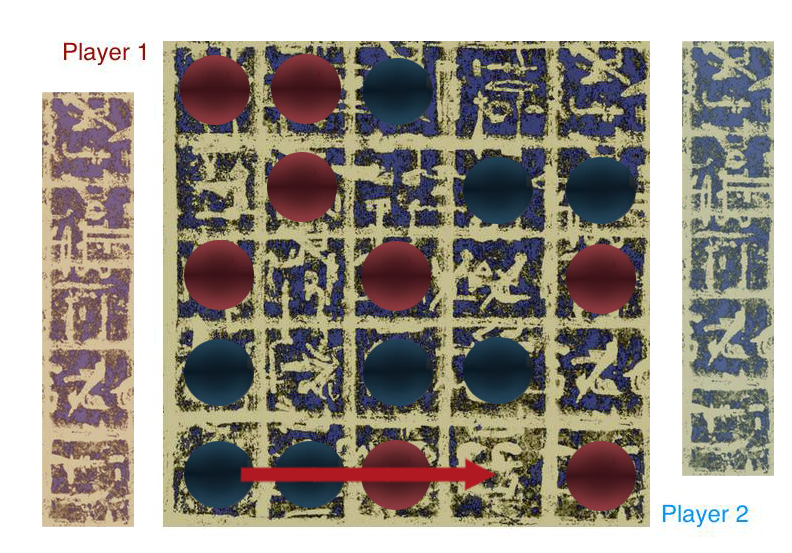
\includegraphics[scale=0.2]{images/push_not_pool.png}
	\caption{\textit{Push} sem que a pedra adversária seja "empurrada" para fora do tabuleiro.}
\endminipage\hfill
\minipage{0.5\textwidth}
 \vspace*{2.3cm}
	\centering
	 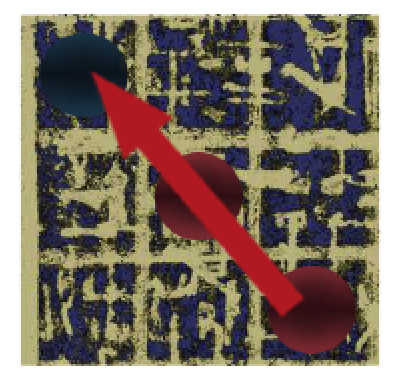
\includegraphics[scale=0.2]{images/push_pool.png} \vspace*{0.3cm}
	\caption{\textit{Push} em que a pedra do adversário é "empurrada" para fora do tabuleiro.}
\endminipage
\end{figure}

\newpage

\begin{figure}[!htb]
	\centering
	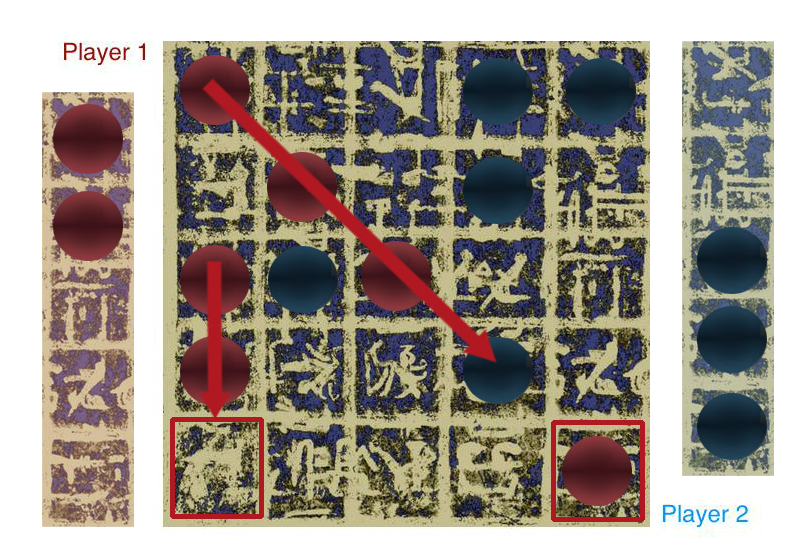
\includegraphics[scale=0.2]{images/invalid_push.png} 
	\caption{Push inválido: nas suas próprias pedras (a); numa célula vazia (b).}
\end{figure}

\textbf{Move}\\

É possível realizar um  \textit{Move} para uma célula vazia em qualquer direção. Se o jogador tentar realizar um \textit{Move} para uma célula ocupada, então é considerado uma jogada inválida.

Se um jogador realizar um \textit{Move} e a sua pedra ficar voluntariamente cercada, esta não é capturada.

\begin{figure}[!htb]
\minipage{0.5\textwidth}
	\centering
  	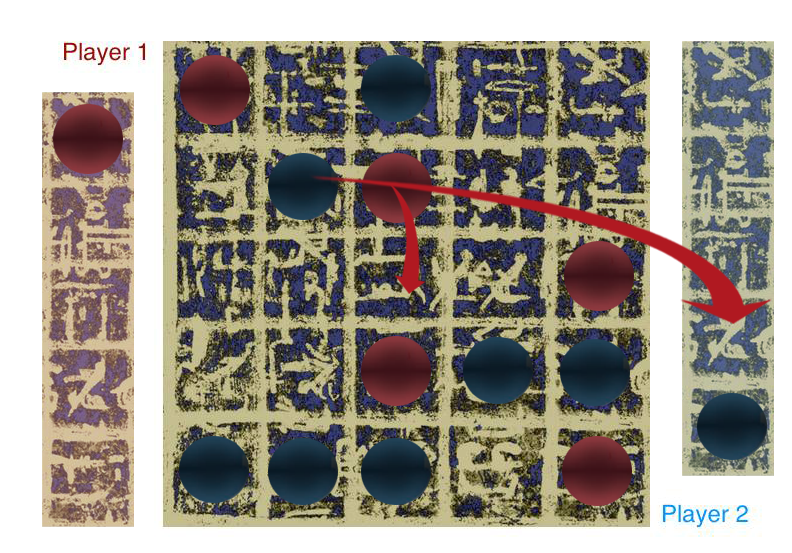
\includegraphics[scale=0.3]{images/move_cap.png} 
	\caption{Pedra azul capturada após um \textit{Move} de uma pedra vermelha.}
\endminipage\hfill
\minipage{0.5\textwidth}
	\vspace*{3.1cm}
	\centering
	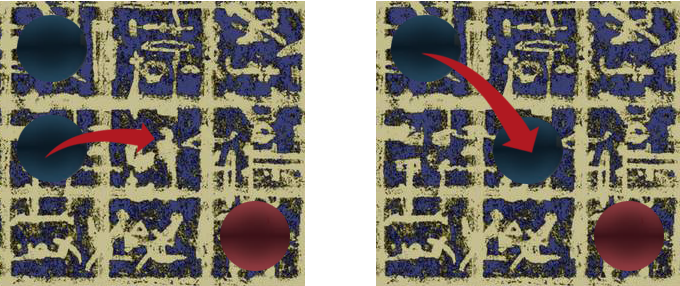
\includegraphics[scale=0.2]{images/valid_invalid_move.png} \vspace*{0.3cm}
	\caption{\textit{Move} válido (a) e um \textit{Move} inválido (b).}
\endminipage
\end{figure}

\textbf{Sacrifice}\\

Um jogador pode sacrificar uma pedra do seu "banco", permanentemente, para poder realizar um \textit{Push} ou um \textit{Move} adicional.\\

% falta imagem para o sacrifice...

\textbf{Capture}\\

Uma pedra fica cercada quando existem pelo menos em duas direções opostas pedras adversárias. Por exemplo se após um \textit{Move} se alguma das pedras adversárias ficar cercada, então esta é capturada e substituída por uma pedra do "banco" do jogador que a capturou.

Após um \textit{Push}, se uma das pedras do jogador atual se move para uma posição que já esta ocupada por uma das suas pedras e fica a cercar uma pedra adversária então é capturada.

Se após um \textit{Push} uma das pedras do adversário fica cercada, então é capturada.

Quando uma pedra adversária é capturada, esta pedra é colocada na \textit{Pool} do adversário e é substituída por outra da \textit{Pool} do jogador que efetuou a jogada.

\begin{figure}[!htb]
	\centering
	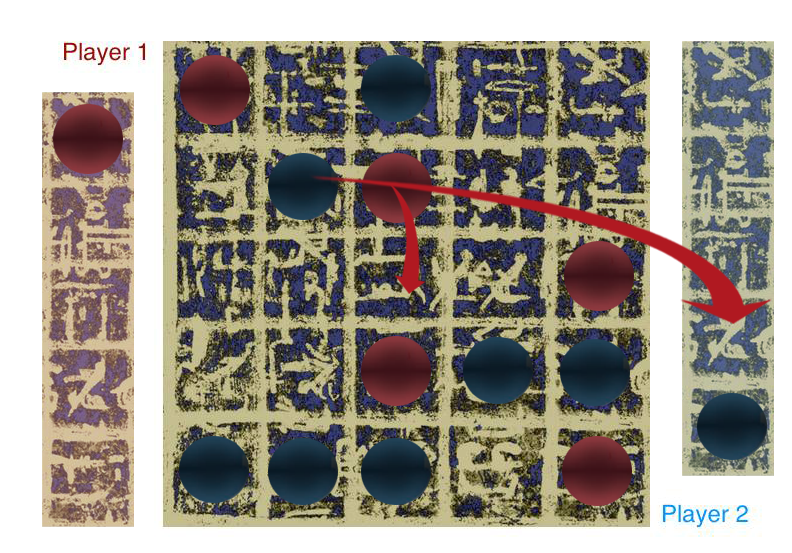
\includegraphics[scale=0.3]{images/move_cap.png} 
	\caption{Pedra azul capturada após um \textit{Move} de uma pedra vermelha.} %melhorar imagem...
\end{figure}

O jogo termina quando o jogador vencedor consegue reduzir para um o número de pedras em jogo do adversário.

%%%%%%%%%%%%%%%%%%%%%%%%%%
\section{Lógica do Jogo}

Descrever o projeto e implementação da lógica do jogo em Prolog, incluindo a forma de representação do estado do tabuleiro e sua visualização, execução de movimentos, verificação do cumprimento das regras do jogo, determinação do final do jogo e cálculo das jogadas a realizar pelo computador utilizando diversos níveis de jogo. Sugere-se a estruturação desta secção da seguinte forma:

\subsection{Representação do Estado do Jogo}

O tabuleiro é representado por uma lista de listas  $L = \{L_1, L_2, ... , L_n\} , n > 0  \wedge n$ é múltiplo de $5$, em que $n$ é a dimensão do tabuleiro. \par
Com o predicado \texttt{make\_board} é possível criar um tabuleiro (\textit{Board}) com um tamanho \textit{Size}. Para isso o \texttt{make\_board} utiliza o predicado \texttt{make\_line} para criar uma linha e depois usa o \texttt{make\_board} recursivamente. De forma a tornar mais clara a visualização do tabuleiro de jogo, após criá-lo com o \texttt{make\_board} utiliza-se o predicado \texttt{print\_board} que o imprime no ecrã.

\begin{figure}[!htb]
	\centering
	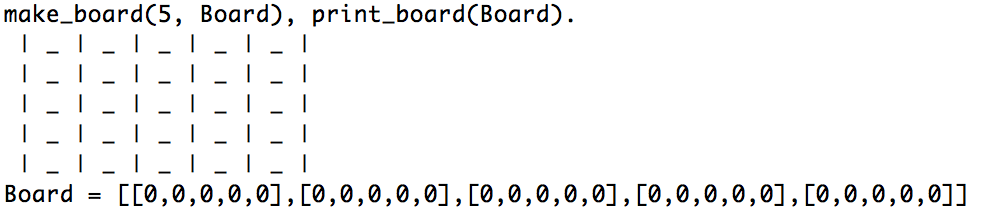
\includegraphics[scale=0.45]{images/make_board.png}
	\caption{Estado inicial do jogo.}
\end{figure}

A figura acima demonstra o estado do tabuleiro na sua fase inicial, sem nenhuma célula preenchida. De uma forma mais visual, segue-se abaixo uma figura demonstrativa do tabuleiro.

\begin{figure}[!htb]
	\centering
	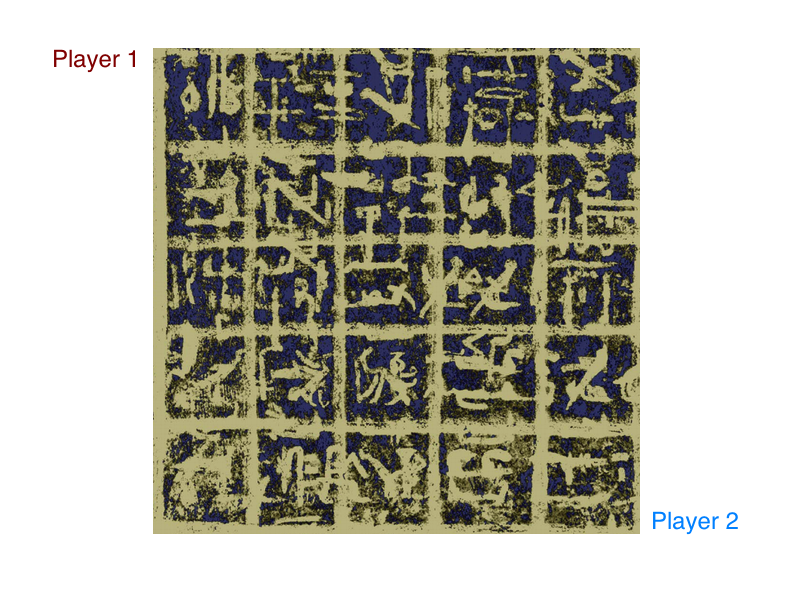
\includegraphics[scale=0.3]{images/board.png}
	\caption{Tabuleiro de jogo.}
\end{figure}

O jogador pode realizar cada uma das três jogadas possíveis: \textit{Push}, \textit{Move} e \textit{Sacrifice}. Para o \textit{Push} é usado o predicado \texttt{push(Stone\_src, Stone\_dst, Dir, Board)}, onde \texttt{Stone\_src} e \texttt{Stone\_dst} são as coordenadas x-y (separadas por um traço) das pedras inicial e destino, \texttt{Dir} é a direção do \textit{Push} e pode ter os valores: 0 (cima), 1 (direita), 2 (baixo) ou 3 (esquerda) e \texttt{Board} é o tabuleiro que é retornado após o \textit{Push}.

\begin{figure}[!htb]
	\centering
	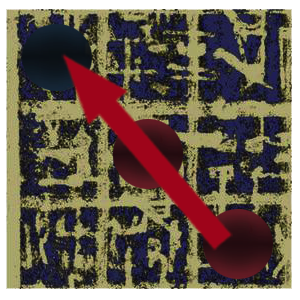
\includegraphics[scale=0.2]{images/push.png}
	\caption{Exemplo de um \textit{Push}.}
\end{figure}

\newpage

Para o \textit{Move} é usado o predicado \texttt{move(Stone\_src, Cell\_dst, Board)}, onde \texttt{Stone\_src} é a pedra que se pretende mover, \texttt{Cell\_dst} é a célula de destino e o \texttt{Board} é o tabuleiro que é retornado.

\begin{figure}[!htb]
	\centering
	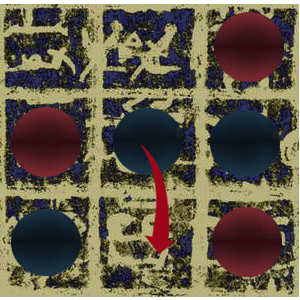
\includegraphics[scale=0.3]{images/move.png}
	\caption{Exemplo de um \textit{Move}.}
\end{figure}

Para o \textit{Sacrifice} é usado o predicado \texttt{sacrifice(Stone, Board)}, onde \texttt{Stone} é a pedra que se pretende sacrificar e o \texttt{Board} é o tabuleiro que é retornado.

\begin{figure}[!htb]
	\centering
	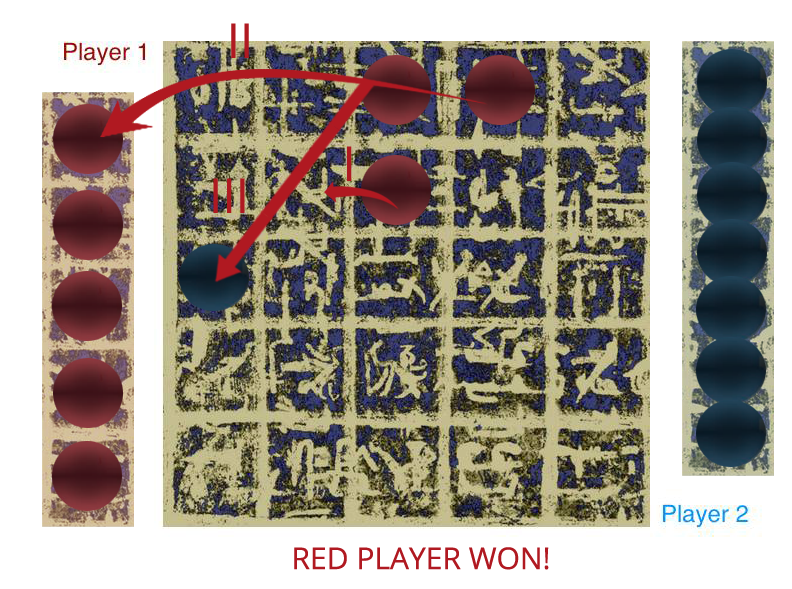
\includegraphics[scale=0.3]{images/sacrifice.png}
	\caption{Exemplo de um \textit{Sacrifice} (II).}
\end{figure}

Existe ainda um predicado \texttt{moveToPool(Stone, Player, Pool)} que move uma uma pedra (\texttt{Stone}) para o "banco" de um dado jogador (\texttt{Player}) retorna o "banco" do jogador (\texttt{Pool}) após a pedra ter sido movida.

\begin{figure}[!htb]
	\centering
	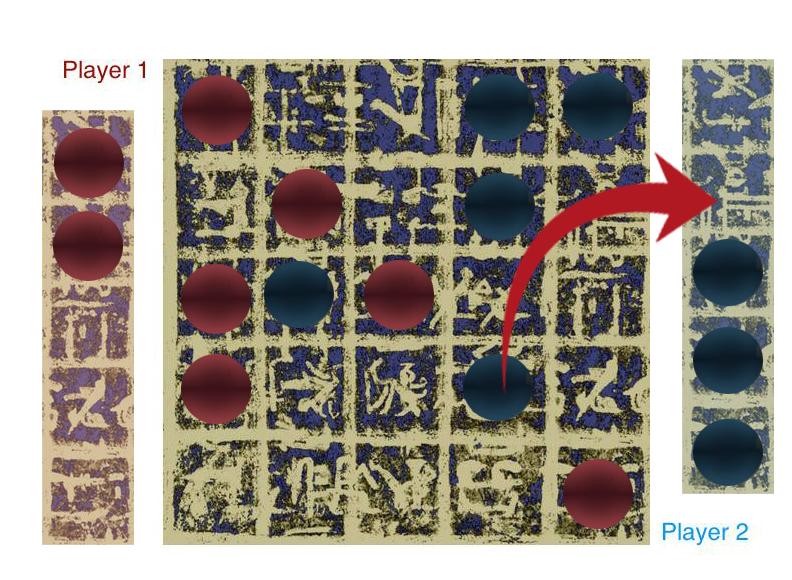
\includegraphics[scale=0.2]{images/pool.png}
	\caption{Exemplo de uma pedra a ser colocada no "banco" de um jogador.}
\end{figure}

%----------------------------------------------------------------------------------------------------------------------------------------------------------------------
\section{Visualização do Tabuleiro}

A cor das pedras dos jogadores são representadas pelos carateres \texttt{O} para as pedras do jogador 1 (azuis) e \texttt{X} para as pedras do jogador 2 (vermelhos), sendo que as casa vazias não têm um caratér específico para a sua representação.

Os predicados utilizados para construir e visualizar o tabuleiro são:

\begin{itemize}
	\item \texttt{translate/2} - Traduz na lista de listas o significado de cada número (0 para casas vazias, 1 para peças do jogador 1 e 2 para peças do jogador 2)
	\item \texttt{make\_line/2} - Gera uma linha do tabuleiro
	\item \texttt{make\_board/2} - Gera um tabuleiro de jogo com o tamanho especificado
	\item \texttt{draw\_board/2 e seus auxiliares} - Predicados para imprimir o tabuleiro
	\item \texttt{draw\_border/1} - Predicado para imprimir o limite do tabuleiro
	\item \texttt{draw\_board\_lines/2} - Predicado que imprime uma linha do tabuleiro
	\item \texttt{draw\_pools/2} - Predicado que imprime as \textit{pools} dos jogadores
\end{itemize}

\begin{figure}[!htb]
	\centering
	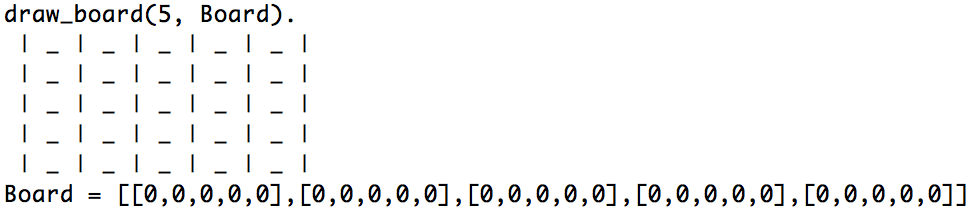
\includegraphics[scale=0.8]{images/draw_board.png}
	\caption{Exemplo de chamada do predicado \texttt{draw\_board} para um tamanho de 5x5}
\end{figure}

Numa fase já final do jogo, o tabuleiro poderá atingir um ponto com o seguinte o formato:

\begin{figure}[!htb]
	\centering
	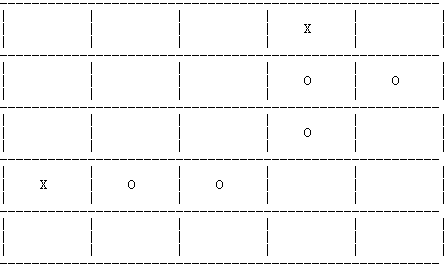
\includegraphics[scale=0.6]{images/board_prolog.png}
	\caption{Exemplo de fase final do jogo.}
\end{figure}

De uma forma mais visual, segue-se abaixo uma figura ilustrativa da fase respetiva do tabuleiro.

\begin{figure}[!htb]
	\centering
	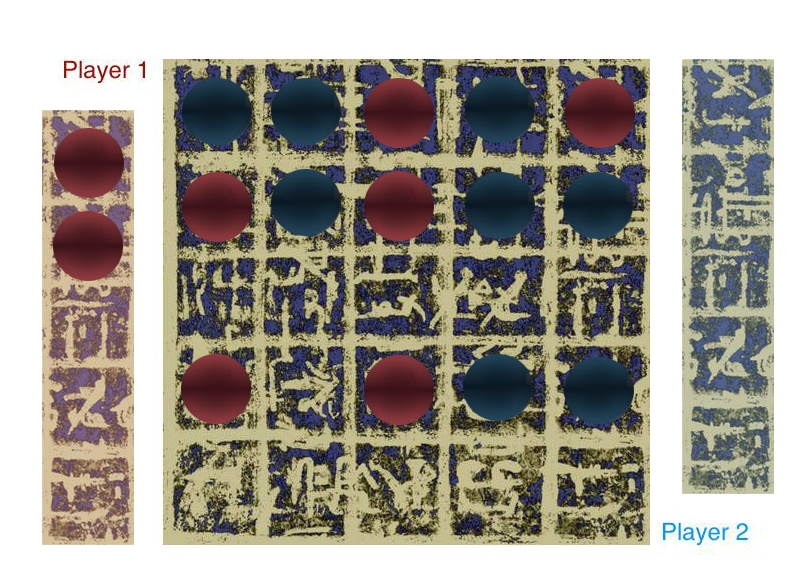
\includegraphics[scale=0.6]{images/board_inter.png}
	\caption{Forma mais visual de uma fase intermédia do jogo.}
\end{figure}

\newpage

%----------------------------------------------------------------------------------------------------------------------------------------------------------------------

\subsection{Lista de Jogadas Válidas} 

A lista de jogadas possíveis e válidas não foi feita porque o jogo ficou apenas completo com o modo computador vs computador, pelo que não era necessário a listagem de jogadas válidas, tendo apenas sido feito as verificações antes de executar cada jogada para ver se a jogada é de facto ou não válida (verificar se a casa para onde se vai mover está vazia, verificar se a peça selecionada é do jogador em questão, verificar se o movimento não mete a peça selecionada numa posição inválida no tabuleiro, etc).

\subsection{Execução de Jogadas} 

Como foi dito em cima existem três tipos de jogadas diferentes:

	\texttt{Push} - A jogada de \textit{push} utiliza os seguintes predicados para a sua execução:
	\begin{itemize}
		\item \textit{push\_n/7} - Verifica se a peça selecionada é do jogador e se assim for executa o push na direção norte.
		\item \textit{push\_s/7} - Verifica se a peça selecionada é do jogador e se assim for executa o push na direção sul.
		\item \textit{push\_e/7} - Verifica se a peça selecionada é do jogador e se assim for executa o push na direção este.
		\item \textit{push\_w/7} - Verifica se a peça selecionada é do jogador e se assim for executa o push na direção oeste.
		\item \textit{push\_ne/7} - Verifica se a peça selecionada é do jogador e se assim for executa o push na direção nordeste.
		\item \textit{push\_nw/7} - Verifica se a peça selecionada é do jogador e se assim for executa o push na direção noroeste.
		\item \textit{push\_sw/7} - Verifica se a peça selecionada é do jogador e se assim for executa o push na direção sudoeste.
		\item \textit{push\_se/7} - Verifica se a peça selecionada é do jogador e se assim for executa o push na direção sudeste.
		\item \textit{valid\_push/4} - Verifica se o push efetuado é válido ou não.
	\end{itemize}
	\texttt{Move} - A jogada de \textit{move} utiliza os seguintes predicados para a sua execução:
	\begin{itemize}
		\item \textit{move/8} - Executa a jogada de \textit{move}, depende dos predicados listados em baixo.
		\item \textit{getStone/4} - Retorna uma peça com as coordenadas dadas do tabuleiro.
		\item \textit{get\_position\_from\_orientation/5} - Dada uma posição do tabuleiro e uma orientação retorna as coordenadas da posição que se encontra na direção da orientação passada.
		\item \textit{check\_empty\_cell/3} - Verifica se no tabuleiro, a casa com as coordenadas passadas se encontra vazia.
		\item \textit{move\_aux/6} - Predicado auxiliar para efetuar a jogada de \textit{move}.
		\item \textit{check\_capture\_status/6} - Verifica se existe captura de peças adversárias após o \textit{move}.
		\item \textit{remove\_captured\_stones/6} - Se existerem peças capturadas, este predicado remove-as do tabuleiro e move-as para a \textit{pool} do jogador em questão.
	\end{itemize}
	\texttt{Sacrifice} - A jogada de \textit{sacrifice} permite ao jogador sacrificar uma das suas peças em jogo (no tabuleiro) para ganhar uma jogada extra (\textit{move} ou \textit{push}), no entanto não ficou implementada por falta de tempo.

\subsection{Avaliação do Tabuleiro} 

Não foi feita a avaliação do  tabuleiro visto que o modo de computador não ficou completo, pelo que não era necessário para o modo jogador vs jogador a avaliação de potenciais jogadas.

\subsection{Final do Jogo} 

O jogo termina quando o número de peças em jogo de um jogador é reduzido a uma unidade. Esta verificação é feita dentro do ciclo de cada jogada, após a sua execução através de dois predicados adicionais do loop de jogo descritos em baixo:

	\begin{figure}[!htb]
	\centering
	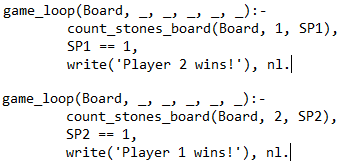
\includegraphics[scale=0.8]{images/game_loop.png}
	\caption{Predicados para verificação do final do jogo.}
\end{figure}

Se o número de peças de um dos jogadores for reduzido a um após uma jogada então na próxima iteração do ciclo o jogo terminará!

\subsection{Jogada do Computador} 

Não implementado devido ao modo de computador não ter sido feito.


%%%%%%%%%%%%%%%%%%%%%%%%%%
\section{Interface com o Utilizador}

A interface com o utilizador é feita pela consola do SICSTUS via texto.
\newline

Para iniciar o jogo usa-se o predicado \textit{initialize\_board(Board, BoardSize, ResultBoard)} que começa o jogo segundo as
regras descritas em cima. Durante o jogo é impresso o tabuleiro, é perguntado ao utilizador
que jogadas pretende efetuar utilizando para tal coordenadas iniciais e finais da peça para a qual se pretende efetuar a jogada.


%%%%%%%%%%%%%%%%%%%%%%%%%%
\section{Conclusões}

O trabalho foi realizado em conjunto em horário fora de aulas.
\newline

Foi desenvolvido em Sicstus em ambiente Windows e Mac.
\newline

O trabalho fez com que conseguíssemos melhorar a nossa capacidade de
programação em lógica, fazendo-nos ter os conhecimentos necessários caso nos sejam
propostos desafios mais complexos.
O jogo não ficou completo totalmente, estando a faltar algumas funcionalidades
como a jogada de \textit{sacrifice}, e faltando ainda os modos de AI vs AI e Humano vs AI, sendo que
neste momento o jogo apenas suporta os jogos entre duas entidades humanas. No futuro e
com mais tempo e de forma bem melhor organizada da nossa parte gostaríamos de desenvolver uma interface mais acessível e intuitiva,
acabar as funcionalidades em falta e tentar implementar uma AI que ofereça um bom
desafio.


\clearpage
\addcontentsline{toc}{section}{Bibliografia}
\renewcommand\refname{Bibliografia}
\bibliographystyle{plain}
\bibliography{myrefs}

\newpage
\appendix
\section{Nome do Anexo}
Código Prolog implementado devidamente comentado e outros elementos úteis que não sejam essenciais ao relatório.\newline
	
	
	Ficheiro \texttt{board.pl}
	\begin{lstlisting}
	
		
		/*

TRANSLATE - Convert a number to figure (_, O or X)
The first parameter is a possible board cell number.
The second parameter is the respective translation to a figure.

*/

translate(0, ' ').

translate(1, 'O').

translate(2, 'X').

/*

MAKE_LINE - Make a game board line
Size - The size of the line
Line - Line to be returned

*/

make_line(0, []).

make_line(Size, Line):- 
        NewSize is Size-1,
        make_line(NewSize, NewLine), 
        append(NewLine, [0], Line).

/*

MAKE_BOARD - Make a board of size NxN
Size - Board's size
Counter - Size's counter (starts in 0 and ends when Size = Counter)
Board - Game board of size NxN

*/

make_board(Size, Board):- 
        make_board(Size, 0, Board), !.
                
make_board(S, S, []).

make_board(Size, Counter, Board):- 
        Size > Counter,
        NewCounter is Counter + 1,
        make_line(Size, Line),
        make_board(Size, NewCounter, NewBoard),
        append(NewBoard, [Line], Board).

/*

DRAW_BOARD - Make board of size NxN and print it
Size - Board's size
Board - Game board of size NxN

*/

draw_board(Size, Board) :- 
        draw_border(Size),
        draw_board_lines(Size, Board),
        nl.

draw_board(Size, Board, Pool, Player) :- 
        Player == 1, 
        draw_border(Size),
        draw_board_lines(Size, Board), nl,
        write('Player 1 Pool'), nl,
        draw_pools(Pool,Size), nl.

draw_board(Size, Board, Pool, Player) :- 
        Player == 2, 
        draw_border(Size),
        draw_board_lines(Size, Board), nl,
        write('Player 2 Pool'), nl,
        draw_pools(Pool,Size), nl.

draw_board(Size, Board, Pool1, Pool2) :- 
        draw_border(Size),
        draw_board_lines(Size, Board), nl,
        write('Player 1 Pool'), nl,
        draw_pools(Pool1,Size), nl,
        write('Player 2 Pool'), nl,
        draw_pools(Pool2,Size).

/*

DRAW_BORDER - Draw board limit
Size - Board's size
 
*/

draw_border(0):- 
        nl, !.

draw_border(Size):- 
        NewSize is Size - 1,
        write('-----------'),
        draw_border(NewSize).

/*

DRAW_BOARD_LINES - Draw each board line
Size - Board's size
Board - Game board of size NxN
      
*/

draw_board_lines(_, []).

draw_board_lines(Size, [H|T]):- 
        draw_empty(Size),
        draw_line(Size, H),
        draw_empty(Size),
        draw_border(Size),
        draw_board_lines(Size, T).

/*

DRAW_EMPTY - Draw the board line without the characters
Size - Board's size
      
*/

draw_empty(0):- 
        write('|'), nl, !.

draw_empty(Size):- 
        write('|          '),
        Size > 0,
        NewSize is Size-1,
        draw_empty(NewSize).

/*
   
DRAW_LINE - Draw the board line with the characters
Size - Board's size
Board - Game board of size NxN
   
*/

draw_line(0,_):- 
        write('|'), nl, !.

draw_line(Size, [H|T]):- 
        NewSize is Size-1,
        write('|    '),
        translate(H,Char),
        write(Char),
        write('     '),
        draw_line(NewSize, T).

/*
  
DRAW_POOLS - draw each players pool
Stones - List of players' stones
Size - Board's size
    
*/

draw_pools(Stones, Size):- 
        PoolSize is round((8/5)*Size),
        draw_border(PoolSize),
        draw_empty(PoolSize),
        draw_line(PoolSize, Stones),
        draw_empty(PoolSize),
        draw_border(PoolSize), nl,!.
                           


/* ---------------------------------------------------
   |         |         |         |         |         |  
   |         |    X    |         |    O    |    O    | 
   |         |         |         |         |         | 
   ---------------------------------------------------
   |         |         |         |         |         |  
   |    O    |         |    X    |    X    |    X    | 
   |         |         |         |         |         | 
   ---------------------------------------------------
   |         |         |         |         |         |  
   |    X    |         |         |    O    |    X    | 
   |         |         |         |         |         | 
   ---------------------------------------------------
   |         |         |         |         |         |  
   |         |         |    O    |    O    |         | 
   |         |         |         |         |         | 
   ---------------------------------------------------
   |         |         |         |         |         |  
   |    X    |    X    |    O    |    O    |         | 
   |         |         |         |         |         | 
   ---------------------------------------------------
   
   Player 1 Pool
   -----------------------------------------------------------------------
   |         |         |         |         |         |         |         |
   |         |         |         |         |         |         |         |
   |         |         |         |         |         |         |         |
   -----------------------------------------------------------------------
   
   Player 2 Pool
   -----------------------------------------------------------------------
   |         |         |         |         |         |         |         |
   |         |         |         |         |         |         |         |
   |         |         |         |         |         |         |         |
   -----------------------------------------------------------------------
   
   | _ | x | _ | o | o |
   | o | _ | x | x | x |
   | x | _ | _ | o | x |
   | _ | _ | o | o | _ |
   | x | x | o | o | _ |
    
   
   _ - 0
   o - 1
   x - 2
*/
	\end{lstlisting}
	
	Ficheiro \texttt{movements.pl}
	
	\begin{lstlisting}
	/*
   ****** PUSH ******
*/

% --- PUSH_N ---

push_n(Board, Player, X, Y, Count, NewX, Y):- 
        nth1(X, Board, Line),
        nth1(Y, Line, Stone),
        Stone == Player,
        XX is X-1,
        push_n(Board, Player, XX, Y, NewCount, NewX, Y),
        Count is NewCount+1.

push_n(_, _, X, Y, 0, NewX, Y):- 
        X \= 0,
        NewX is X.

push_n(_, _, X, Y, 0, NewX, Y):- 
        X == 0,
        NewX is X+1.

% --- PUSH_S ---

push_s(Board, Player, X, Y, Count, NewX, Y):- 
        nth1(X, Board, Line),
        nth1(Y, Line, Stone),
        Stone == Player,
        XX is X+1,
        push_s(Board, Player, XX, Y, NewCount, NewX, Y),
        Count is NewCount+1.

push_s(Board, _, X, Y, 0, NewX, Y):- 
        nth1(X, Board, Line),
        length(Line,L),
        X \= L,
        NewX is X.

push_s(Board, _, X, Y, 0, NewX, Y):- 
        nth1(X, Board, Line),
        length(Line,L),
        X == L,
        NewX is X.

% --- PUSH_E ---

push_e(Board, Player, X, Y, Count, X, NewY):- 
        nth1(X, Board, Line),
        nth1(Y, Line, Stone),
        Stone == Player,
        YY is Y+1,
        push_e(Board, Player, X, YY, NewCount, X, NewY),
        Count is NewCount+1.

push_e(Board, _, X, Y, 0, X, NewY):- 
        nth1(X, Board, Line),
        length(Line,L),
        Y \= L,
        NewY is Y.

push_e(Board, _, X, Y, 0, X, NewY):- 
        nth1(X, Board, Line),
        length(Line,L),
        Y == L,
        NewY is Y.

% --- PUSH_W ---

push_w(Board, Player, X, Y, Count, X, NewY):- 
        nth1(X, Board, Line),
        nth1(Y, Line, Stone),
        Stone == Player,
        YY is Y-1,
        push_w(Board, Player, X, YY, NewCount, X, NewY),
        Count is NewCount+1.

push_w(_, _, X, Y, 0, X, NewY):- 
        Y \= 0,
        NewY is Y.

push_w(_, _, X, Y, 0, X, NewY):- 
        Y == 0,
        NewY is Y.

% --- PUSH_NE ---

push_ne(Board, Player, X, Y, Count, NewX, NewY):- 
        nth1(X, Board, Line),
        nth1(Y, Line, Stone),
        Stone == Player,
        XX is X-1,
        YY is Y+1,
        push_ne(Board, Player, XX, YY, NewCount, NewX, NewY),
        Count is NewCount+1.

push_ne(_, _, X, Y, 0, NewX, NewY):- 
        X == 0,
        NewX is X+1,
        NewY is Y-1.

push_ne(_, _, X, Y, 0, NewX, NewY):- 
        NewX is X,
        NewY is Y.

% --- PUSH_SW ---

push_sw(Board, Player, X, Y, Count, NewX, NewY):- 
        nth1(X, Board, Line),
        nth1(Y, Line, Stone),
        Stone == Player,
        XX is X+1,
        YY is Y-1,
        push_sw(Board, Player, XX, YY, NewCount, NewX, NewY),
        Count is NewCount+1.

push_sw(_, _, X, Y, 0, NewX, NewY):- 
        Y == 0,
        NewX is X-1,
        NewY is Y+1.

push_sw(_, _, X, Y, 0, NewX, NewY):- 
        NewX is X,
        NewY is Y.

% --- PUSH_NW ---

push_nw(Board, Player, X, Y, Count, NewX, NewY):- 
        nth1(X, Board, Line),
        nth1(Y, Line, Stone),
        Stone == Player,
        XX is X-1,
        YY is Y-1,
        push_nw(Board, Player, XX, YY, NewCount, NewX, NewY),
        Count is NewCount+1.

push_nw(_, _, X, Y, 0, NewX, NewY):- 
        X \= 0,
        NewX is X,
        NewY is Y.

push_nw(_, _, X, Y, 0, NewX, NewY):- 
        X == 0,
        NewX is X+1,
        NewY is Y+1.

% --- PUSH_SE ---

push_se(Board, Player, X, Y, Count, NewX, NewY):- 
        nth1(X, Board, Line),
        nth1(Y, Line, Stone),
        Stone == Player,
        XX is X+1,
        YY is Y+1,
        push_se(Board, Player, XX, YY, NewCount, NewX, NewY),
        Count is NewCount+1.

push_se(Board, _, X, Y, 0, NewX, NewY):- 
        nth1(X, Board, Line),
        length(Line,L),
        X \= L,
        NewX is X,
        NewY is Y.

push_se(Board, _, X, Y, 0, NewX, NewY):- 
        nth1(X, Board, Line),
        length(Line,L),
        X == L,
        NewX is X-1,
        NewY is Y-1.

% --- VALID_PUSH ---

valid_push(Board, NextX, NextY, Valid):- 
        nth1(NextX, Board, NextLine),
        nth1(NextY, NextLine, NextStone),
        NextStone == 0,
        Valid is 1, !.

% --- VALID_PUSH N ---

valid_push(Board, NextX, NextY, Valid, Orientation):- 
        nth1(NextX, Board, NextLine),
        nth1(NextY, NextLine, _),
        Orientation == 'n',
        NextX == 1,
        Valid is 1, !.

% --- VALID_PUSH S ---

valid_push(Board, NextX, NextY, Valid, Orientation):- 
        nth1(NextX, Board, NextLine),
        nth1(NextY, NextLine, _),
        length(NextLine, L),
        Orientation == 's',
        NextX == L,
        Valid is 1, !.

% --- VALID_PUSH E ---

valid_push(Board, NextX, NextY, Valid, 'e'):- 
        nth1(NextX, Board, NextLine),
        nth1(NextY, NextLine, _),
        length(NextLine, L),
        NextY == L,
        Valid is 1, !.     
      
% --- VALID_PUSH W ---

valid_push(Board, NextX, NextY, Valid, 'w'):- 
        nth1(NextX, Board, NextLine),
        nth1(NextY, NextLine, _),
        NextY == 1,
        Valid is 1, !.

% --- VALID_PUSH NE ---

valid_push(Board, NextX, NextY, Valid, 'ne'):- 
        nth1(NextX, Board, NextLine),
        nth1(NextY, NextLine, _),
        length(NextLine, L),
        NextY == L,
        Valid is 1, !.

valid_push(_, NextX, _, Valid, 'ne'):- 
        NextX == 1,
        Valid is 1, !.

% --- VALID_PUSH SE ---

valid_push(Board, NextX, NextY, Valid, 'se'):- 
        nth1(NextX, Board, NextLine),
        nth1(NextY, NextLine, _),
        length(NextLine, L),
        NextX == L,
        Valid is 1, !.

valid_push(Board, NextX, NextY, Valid, 'se'):- 
        nth1(NextX, Board, NextLine),
        nth1(NextY, NextLine, _),
        length(NextLine, L),
        NextY == L,
        Valid is 1, !.

% --- VALID_PUSH SW ---

valid_push(Board, NextX, NextY, Valid, 'sw'):- 
        nth1(NextX, Board, NextLine),
        nth1(NextY, NextLine, _),
        length(NextLine, L),
        NextX == L,
        Valid is 1, !.

valid_push(_, _, NextY, Valid, 'sw'):- 
        NextY == 1,
        Valid is 1, !.

% --- VALID_PUSH NW ---

valid_push(Board, NextX, NextY, Valid, 'nw'):- 
        nth1(NextX, Board, NextLine),
        nth1(NextY, NextLine, _),
        NextX == 1,
        Valid is 1, !.

valid_push(Board, NextX, NextY, Valid, 'nw'):- 
        nth1(NextX, Board, NextLine),
        nth1(NextY, NextLine, _),
        NextY == 1,
        Valid is 1, !.

% --- BEFORE_LIST ---

before_list(L, N, R):- 
        before_list(L, N, 0, R).

before_list([H|T], N, Counter, R):- 
        N > Counter - 1,
        NewCounter is Counter + 1,
        before_list(T, N, NewCounter, LR),
        append([H], LR, R).

before_list(_, N, N, []).

% --- AFTER_LIST ---

after_list(L, N, R):- 
        after_list(L, N, 0, R).

after_list([_|T], N, Counter, R):- 
        N >= Counter,
        NewCounter is Counter + 1,
        after_list(T, N, NewCounter, R).

after_list([H|T], N, Counter, R):- 
        Counter > N,
        NewCounter is Counter + 1,
        after_list(T, N, NewCounter, LR),
        append([H], LR, R).

% --- REMOVE_LAST ---

remove_last([_], []).

remove_last([H|T], [H|NewList]) :- 
        remove_last(T, NewList).

remove_first([_|T], T).

% --- UPDATE_BOARD_N ---

update_board_n(Board, X, Y, 1, NewBoard):- 
        replace(Board, X, Y, 0, NewBoard).

update_board_n(Board, X, Y, NumStones, Result):- 
        NewX is X-NumStones,
        XX is NewX+1,
        nth1(XX, Board, Line2),
        nth1(Y, Line2, Stone2),
        replace(Board, NewX, Y, Stone2, NewBoard), 
        NewNumStones is NumStones-1,
        update_board_n(NewBoard, X, Y, NewNumStones, Result).

% --- UPDATE_BOARD_S ---

update_board_s(Board, X, Y, 1, NewBoard):- 
        replace(Board, X, Y, 0, NewBoard).

update_board_s(Board, X, Y, NumStones, Result):- 
        NewX is X+NumStones,
        XX is NewX-1,
        nth1(XX, Board, Line2),
        nth1(Y, Line2, Stone2),
        replace(Board, NewX, Y, Stone2, NewBoard), 
        NewNumStones is NumStones-1,
        update_board_s(NewBoard, X, Y, NewNumStones, Result).

% --- UPDATE_BOARD_E ---

update_board_e(Board, X, Y, 1, NewBoard):- 
        replace(Board, X, Y, 0, NewBoard).

update_board_e(Board, X, Y, NumStones, Result):- 
        NewY is Y+NumStones,
        YY is NewY-1,
        nth1(X, Board, Line2),
        nth1(YY, Line2, Stone2),
        replace(Board, X, NewY, Stone2, NewBoard), 
        NewNumStones is NumStones-1,
        update_board_e(NewBoard, X, Y, NewNumStones, Result).

% --- UPDATE_BOARD_W ---

update_board_w(Board, X, Y, 1, NewBoard):- 
        replace(Board, X, Y, 0, NewBoard).

update_board_w(Board, X, Y, NumStones, Result):- 
        NewY is Y-NumStones,
        YY is NewY+1,
        nth1(X, Board, Line2),
        nth1(YY, Line2, Stone2),
        replace(Board, X, NewY, Stone2, NewBoard), 
        NewNumStones is NumStones-1,
        update_board_w(NewBoard, X, Y, NewNumStones, Result).

% --- UPDATE_BOARD_NE ---

update_board_ne(Board, X, Y, 1, NewBoard):- 
        replace(Board, X, Y, 0, NewBoard).

update_board_ne(Board, X, Y, NumStones, Result):- 
        NewX is X-NumStones,
        NewY is Y+NumStones,
        XX is NewX+1,
        YY is NewY-1,
        nth1(XX, Board, Line2),
        nth1(YY, Line2, Stone2),
        replace(Board, NewX, NewY, Stone2, NewBoard), 
        NewNumStones is NumStones-1,
        update_board_ne(NewBoard, X, Y, NewNumStones, Result).

% --- UPDATE_BOARD_SW ---

update_board_sw(Board, X, Y, 1, NewBoard):- replace(Board, X, Y, 0, NewBoard).

update_board_sw(Board, X, Y, NumStones, Result):- 
        NewX is X+NumStones,
        NewY is Y-NumStones,
        XX is NewX-1,
        YY is NewY+1,
        nth1(XX, Board, Line2),
        nth1(YY, Line2, Stone2),
        replace(Board, NewX, NewY, Stone2, NewBoard), 
        NewNumStones is NumStones-1,
        update_board_sw(NewBoard, X, Y, NewNumStones, Result).

% --- UPDATE_BOARD_NW ---

update_board_nw(Board, X, Y, 1, NewBoard):- 
        replace(Board, X, Y, 0, NewBoard).

update_board_nw(Board, X, Y, NumStones, Result):- 
        NewX is X-NumStones,
        NewY is Y-NumStones,
        XX is NewX+1,
        YY is NewY+1,
        nth1(XX, Board, Line2),
        nth1(YY, Line2, Stone2),
        replace(Board, NewX, NewY, Stone2, NewBoard), 
        NewNumStones is NumStones-1,
        update_board_nw(NewBoard, X, Y, NewNumStones, Result).

% --- UPDATE_BOARD_SE ---

update_board_se(Board, X, Y, 1, NewBoard):- 
        replace(Board, X, Y, 0, NewBoard).

update_board_se(Board, X, Y, NumStones, Result):- 
        NewX is X+NumStones,
        NewY is Y+NumStones,
        XX is NewX-1,
        YY is NewY-1,
        nth1(XX, Board, Line2),
        nth1(YY, Line2, Stone2),
        replace(Board, NewX, NewY, Stone2, NewBoard), 
        NewNumStones is NumStones-1,
        update_board_se(NewBoard, X, Y, NewNumStones, Result).

% --- GET_OP_PLAYER ---

get_op_player(Player, Opposite):- 
        Opposite is 2 // Player.

% --- ADD_TO_POOL ---

add_to_pool([], _, 1, []).

add_to_pool([PoolH|PoolT], Stone, Count, NewPool):- 
        PoolH == 0,
        Count == 0,
        add_to_pool(PoolT, Stone, 1, TmpPool),
        append([Stone], TmpPool, NewPool).

add_to_pool([PoolH|PoolT], Stone, Count, NewPool):- 
        add_to_pool(PoolT, Stone, Count, TmpPool),
        append([PoolH], TmpPool, NewPool),!.

% --- PUSH NORTH ---

push(Board, Player, X, Y, 'n', Pool, Pool, Result):- 
        nth1(X, Board, Line),
        nth1(Y, Line, Stone),
        Stone == Player,
        push_n(Board, Player, X, Y, Count, OppositeX, OppositeY),
        get_op_player(Player, Opposite),
        push_n(Board, Opposite, OppositeX, OppositeY, OppositeCount, NextX, NextY),
        Count > OppositeCount,
        OppositeCount > 0,
        valid_push(Board, NextX, NextY, Valid),
        Valid == 1,
        NumStones is Count+OppositeCount,
        update_board_n(Board, X, Y, NumStones, Result).

push(Board, Player, X, Y, 'n', Pool, PoolResult, Result):- 
        nth1(X, Board, Line),
        nth1(Y, Line, Stone),
        Stone == Player,
        push_n(Board, Player, X, Y, Count, OppositeX, OppositeY),
        get_op_player(Player, Opposite),
        push_n(Board, Opposite, OppositeX, OppositeY, OppositeCount, NextX, NextY),
        Count > OppositeCount,
        OppositeCount > 0,
        valid_push(Board, NextX, NextY, Valid, 'n'),
        Valid == 1,
        NumStones is Count+OppositeCount-1,
        update_board_n(Board, X, Y, NumStones, Result),
        add_to_pool(Pool, Opposite, 0, PoolResult).

% --- PUSH SOUTH ---

push(Board, Player, X, Y, 's', Pool, Pool, Result):- 
        nth1(X, Board, Line),
        nth1(Y, Line, Stone),
        Stone == Player,
        push_s(Board, Player, X, Y, Count, OppositeX, OppositeY),
        get_op_player(Player, Opposite),
        push_s(Board, Opposite, OppositeX, OppositeY, OppositeCount, NextX, NextY),
        Count > OppositeCount,
        OppositeCount > 0,
        valid_push(Board, NextX, NextY, Valid),
        Valid == 1,
        NumStones is Count+OppositeCount,
        update_board_s(Board, X, Y, NumStones, Result).

push(Board, Player, X, Y, 's', Pool, PoolResult, Result):- 
        nth1(X, Board, Line),
        nth1(Y, Line, Stone),
        Stone == Player,
        push_s(Board, Player, X, Y, Count, OppositeX, OppositeY),
        get_op_player(Player, Opposite),
        push_s(Board, Opposite, OppositeX, OppositeY, OppositeCount, NextX, NextY),
        NOppositeCount is OppositeCount+1,
        Count > OppositeCount, !,
        NOppositeCount > 0,
        valid_push(Board, NextX, NextY, Valid, 's'),
        Valid == 1,
        NumStones is Count+OppositeCount,
        update_board_s(Board, X, Y, NumStones, Result),
        add_to_pool(Pool, Opposite, 0, PoolResult).

% --- PUSH EAST ---

push(Board, Player, X, Y, 'e', Pool, Pool, Result):- 
        nth1(X, Board, Line),
        nth1(Y, Line, Stone),
        Stone == Player,
        push_e(Board, Player, X, Y, Count, OppositeX, OppositeY),
        get_op_player(Player, Opposite),
        push_e(Board, Opposite, OppositeX, OppositeY, OppositeCount, NextX, NextY),
        Count > OppositeCount,
        OppositeCount > 0,
        valid_push(Board, NextX, NextY, Valid),
        Valid == 1,
        NumStones is Count+OppositeCount,
        update_board_e(Board, X, Y, NumStones, Result).

push(Board, Player, X, Y, 'e', Pool, PoolResult, Result):- 
        nth1(X, Board, Line),
        nth1(Y, Line, Stone),
        Stone == Player,
        push_e(Board, Player, X, Y, Count, OppositeX, OppositeY),
        get_op_player(Player, Opposite),
        push_e(Board, Opposite, OppositeX, OppositeY, OppositeCount, NextX, NextY),
        NOppositeCount is OppositeCount+1,
        Count > OppositeCount, !,
        NOppositeCount > 0,
        SuperNextY is NextY-1,
        valid_push(Board, NextX, SuperNextY, Valid, 'e'),
        Valid == 1,
        NumStones is Count+OppositeCount-1,
        update_board_e(Board, X, Y, NumStones, Result),
        add_to_pool(Pool, Opposite, 0, PoolResult).

% --- PUSH WEST ---

push(Board, Player, X, Y, 'w', Pool, Pool, Result):- 
        nth1(X, Board, Line),
        nth1(Y, Line, Stone),
        Stone == Player,
        push_w(Board, Player, X, Y, Count, OppositeX, OppositeY),
        get_op_player(Player, Opposite),
        push_w(Board, Opposite, OppositeX, OppositeY, OppositeCount, NextX, NextY),
        Count > OppositeCount,
        OppositeCount > 0,
        valid_push(Board, NextX, NextY, Valid),
        Valid == 1,
        NumStones is Count+OppositeCount,
        update_board_w(Board, X, Y, NumStones, Result).

push(Board, Player, X, Y, 'w', Pool, PoolResult, Result):- 
        nth1(X, Board, Line),
        nth1(Y, Line, Stone),
        Stone == Player,
        push_w(Board, Player, X, Y, Count, OppositeX, OppositeY),
        get_op_player(Player, Opposite),
        push_w(Board, Opposite, OppositeX, OppositeY, OppositeCount, NextX, NextY),
        NOppositeCount is OppositeCount+1,
        Count > OppositeCount, !,
        NOppositeCount > 0,
        SuperNextY is NextY+1,
        valid_push(Board, NextX, SuperNextY, Valid, 'w'),
        Valid == 1,
        NumStones is Count+OppositeCount-1,
        update_board_w(Board, X, Y, NumStones, Result),
        add_to_pool(Pool, Opposite, 0, PoolResult).

% --- PUSH NORTHEAST ---

push(Board, Player, X, Y, 'ne', Pool, Pool, Result):- 
        nth1(X, Board, Line),
        nth1(Y, Line, Stone),
        Stone == Player,
        push_ne(Board, Player, X, Y, Count, OppositeX, OppositeY),
        get_op_player(Player, Opposite),
        push_ne(Board, Opposite, OppositeX, OppositeY, OppositeCount, NextX, NextY),
        Count > OppositeCount,
        OppositeCount > 0,
        valid_push(Board, NextX, NextY, Valid),
        Valid == 1,
        NumStones is Count+OppositeCount,
        update_board_ne(Board, X, Y, NumStones, Result).

push(Board, Player, X, Y, 'ne', Pool, PoolResult, Result):- 
        nth1(X, Board, Line),
        nth1(Y, Line, Stone),
        Stone == Player,
        push_ne(Board, Player, X, Y, Count, OppositeX, OppositeY),
        get_op_player(Player, Opposite),
        push_ne(Board, Opposite, OppositeX, OppositeY, OppositeCount, NextX, NextY),
        Count > OppositeCount, !,
        OppositeCount > 0,
        valid_push(Board, NextX, NextY, Valid, 'ne'),
        Valid == 1,
        NumStones is Count+OppositeCount-1,
        update_board_ne(Board, X, Y, NumStones, Result),
        add_to_pool(Pool, Opposite, 0, PoolResult).

% -- PUSH SOUTHEAST ---

push(Board, Player, X, Y, 'se', Pool, Pool, Result):- 
        nth1(X, Board, Line),
        nth1(Y, Line, Stone),
        Stone == Player,
        push_se(Board, Player, X, Y, Count, OppositeX, OppositeY),
        get_op_player(Player, Opposite),
        push_se(Board, Opposite, OppositeX, OppositeY, OppositeCount, NextX, NextY),
        Count > OppositeCount,
        OppositeCount > 0,
        SuperNextX is NextX+1,
        SuperNextY is NextY+1,
        valid_push(Board, SuperNextX, SuperNextY, Valid),
        Valid == 1,
        NumStones is Count+OppositeCount,
        update_board_se(Board, X, Y, NumStones, Result).

push(Board, Player, X, Y, 'se', Pool, PoolResult, Result):- 
        nth1(X, Board, Line),
        nth1(Y, Line, Stone),
        Stone == Player,
        push_se(Board, Player, X, Y, Count, OppositeX, OppositeY),
        get_op_player(Player, Opposite),
        push_se(Board, Opposite, OppositeX, OppositeY, OppositeCount, NextX, NextY),
        NOppositeCount is OppositeCount+1,
        Count > OppositeCount,
        NOppositeCount > 0,
        SuperNextX is NextX+1,
        SuperNextY is NextY+1,
        valid_push(Board, SuperNextX, SuperNextY, Valid, 'se'),
        Valid == 1,
        NumStones is Count+OppositeCount-1,
        update_board_se(Board, X, Y, NumStones, Result),
        add_to_pool(Pool, Opposite, 0, PoolResult).

% --- PUSH SOUTHWEST ---

push(Board, Player, X, Y, 'sw', Pool, Pool, Result):- 
        nth1(X, Board, Line),
        nth1(Y, Line, Stone),
        Stone == Player,
        push_sw(Board, Player, X, Y, Count, OppositeX, OppositeY),
        get_op_player(Player, Opposite),
        push_sw(Board, Opposite, OppositeX, OppositeY, OppositeCount, NextX, NextY),
        Count > OppositeCount,
        OppositeCount > 0,
        valid_push(Board, NextX, NextY, Valid),
        Valid == 1,
        NumStones is Count+OppositeCount,
        update_board_sw(Board, X, Y, NumStones, Result).

push(Board, Player, X, Y, 'sw', Pool, PoolResult, Result):- 
        nth1(X, Board, Line),
        nth1(Y, Line, Stone),
        Stone == Player,
        push_sw(Board, Player, X, Y, Count, OppositeX, OppositeY),
        get_op_player(Player, Opposite),
        push_sw(Board, Opposite, OppositeX, OppositeY, OppositeCount, NextX, NextY),
        Count > OppositeCount, !,
        OppositeCount > 0,
        valid_push(Board, NextX, NextY, Valid, 'sw'),
        Valid == 1,
        NumStones is Count+OppositeCount-1,
        update_board_sw(Board, X, Y, NumStones, Result),
        add_to_pool(Pool, Opposite, 0, PoolResult).

% --- PUSH NORTHWEST ---

push(Board, Player, X, Y, 'nw', Pool, Pool, Result):- 
        nth1(X, Board, Line),
        nth1(Y, Line, Stone),
        Stone == Player,
        push_nw(Board, Player, X, Y, Count, OppositeX, OppositeY),
        get_op_player(Player, Opposite),
        push_nw(Board, Opposite, OppositeX, OppositeY, OppositeCount, NextX, NextY),
        Count > OppositeCount,
        OppositeCount > 0,
        valid_push(Board, NextX, NextY, Valid),
        Valid == 1,
        NumStones is Count+OppositeCount,
        update_board_nw(Board, X, Y, NumStones, Result).

push(Board, Player, X, Y, 'nw', Pool, PoolResult, Result):- 
        nth1(X, Board, Line),
        nth1(Y, Line, Stone),
        Stone == Player,
        push_nw(Board, Player, X, Y, Count, OppositeX, OppositeY),
        get_op_player(Player, Opposite),
        push_nw(Board, Opposite, OppositeX, OppositeY, OppositeCount, NextX, NextY),
        Count > OppositeCount, !,
        OppositeCount > 0,
        valid_push(Board, NextX, NextY, Valid, 'nw'),
        Valid == 1,
        NumStones is Count+OppositeCount-1,
        update_board_nw(Board, X, Y, NumStones, Result),
        add_to_pool(Pool, Opposite, 0, PoolResult).

/*
   ****** MOVE ******
*/

move(Board, 1, X, Y, Orientation, Pool, ResultPool, ResultBoard) :-
        getStone(Board,X,Y,Stone),
        Stone == 1,
        get_position_from_orientation(X, Y, Orientation, NewX, NewY),
        check_empty_cell(Board, NewX, NewY),
        move_aux(Board, X, Y, NewX, NewY, ReturnBoard),
        check_capture_status(ReturnBoard, NewX, NewY, 1, Pool, ResultCaptures),
        remove_captured_stones(ReturnBoard, 2, ResultCaptures, Pool, ResultPool, ResultBoard).

move(Board, 2, X, Y, Orientation, Pool, ResultPool, ResultBoard) :-
        getStone(Board,X,Y,Stone),
        Stone == 2,
        get_position_from_orientation(X, Y, Orientation, NewX, NewY),
        check_empty_cell(Board, NewX, NewY),
        move_aux(Board, X, Y, NewX, NewY, ReturnBoard),
        check_capture_status(ReturnBoard, NewX, NewY, 2, _, ResultCaptures),
        remove_captured_stones(ReturnBoard, 1, ResultCaptures, Pool, ResultPool, ResultBoard).

% --- REMOVE_CAPTURED_STONES ---

remove_captured_stones(Board, _, [], Pool, Pool, Board).

remove_captured_stones(Board, OppositePlayer, [X-Y], Pool, ResultPool, ResultBoard):-
        replace(Board, X, Y, 0, RB),
        add_to_pool(Pool, OppositePlayer, 0, RP),
        remove_captured_stones(RB, OppositePlayer, [], RP, ResultPool, ResultBoard).

remove_captured_stones(Board, OppositePlayer, [X-Y|TC], Pool, ResultPool, ResultBoard):-
        replace(Board, X, Y, 0, RB),
        add_to_pool(Pool, OppositePlayer, 0, RP),
        remove_captured_stones(RB, OppositePlayer, TC, RP, ResultPool, ResultBoard).

% --- CHECK_CAPTURE_STATUS ---

check_capture_status(Board, NewX, NewY, Player, _, ResultCaptures) :- 
        check_capture_status(Board, 'n', NewX, NewY, Player, [], RC1),
        check_capture_status(Board, 's', NewX, NewY, Player, RC1, RC2),
        check_capture_status(Board, 'e', NewX, NewY, Player, RC2, RC3),
        check_capture_status(Board, 'w', NewX, NewY, Player, RC3, RC4),
        check_capture_status(Board, 'nw', NewX, NewY, Player, RC4, RC5),
        check_capture_status(Board, 'ne', NewX, NewY, Player, RC5, RC6),
        check_capture_status(Board, 'sw', NewX, NewY, Player, RC6, RC7),
        check_capture_status(Board, 'se', NewX, NewY, Player, RC7, ResultCaptures), !.

check_capture_status(Board, Orientation, NewX, NewY, Player, CL, RCL) :- 
        getStone(Board, NewX, NewY, PlayerStone),
        PlayerStone == Player,
        get_op_player(Player, OppositePlayer),
        get_position_from_orientation(NewX, NewY, Orientation, CheckX, CheckY),
        getStone(Board, CheckX, CheckY, CheckStone),
        CheckStone == OppositePlayer,
        get_position_from_orientation(CheckX, CheckY, Orientation, SurroundX, SurroundY),
        getStone(Board, SurroundX, SurroundY, PossibleSurroundStone),
        PossibleSurroundStone == Player,
        append(CL, [CheckX-CheckY], RCL).

check_capture_status(Board, Orientation, NewX, NewY, Player, CL, RCL) :- 
        getStone(Board, NewX, NewY, PlayerStone),
        PlayerStone == Player,
        get_position_from_orientation(NewX, NewY, Orientation, CheckX, _),
        CheckX == 0,
        append(CL, [], RCL).
   
check_capture_status(Board, Orientation, NewX, NewY, Player, CL, RCL) :- 
        getStone(Board, NewX, NewY, PlayerStone),
        PlayerStone == Player,
        get_position_from_orientation(NewX, NewY, Orientation, _, CheckY),
        CheckY == 0,
        append(CL, [], RCL).

check_capture_status(Board, Orientation, NewX, NewY, Player, CL, RCL) :- 
        getStone(Board, NewX, NewY, PlayerStone),
        PlayerStone == Player,
        get_position_from_orientation(NewX, NewY, Orientation, CheckX, _),
        CheckX > 0,
        append(CL, [], RCL).

check_capture_status(Board, Orientation, NewX, NewY, Player, CL, RCL) :- 
        getStone(Board, NewX, NewY, PlayerStone),
        PlayerStone == Player,
        get_position_from_orientation(NewX, NewY, Orientation, _, CheckY),
        CheckY > 0,
        append(CL, [], RCL).

check_capture_status(Board, Orientation, NewX, NewY, Player, CL, RCL) :- 
        getStone(Board, NewX, NewY, PlayerStone),
        PlayerStone == Player,
        get_position_from_orientation(NewX, NewY, Orientation, CheckX, _),
        nth1(1,Board,Line),
        length(Line,Size),
        CheckX > Size,
        append(CL, [], RCL).

check_capture_status(Board, Orientation, NewX, NewY, Player, CL, RCL) :- 
        getStone(Board, NewX, NewY, PlayerStone),
        PlayerStone == Player,
        get_position_from_orientation(NewX, NewY, Orientation, _, CheckY),
        nth1(1,Board,Line),
        length(Line,Size),
        CheckY > Size,
        append(CL, [], RCL).

check_capture_status(Board, Orientation, NewX, NewY, Player, CL, CL):-
        getStone(Board, NewX, NewY, PlayerStone),
        PlayerStone == Player,
        get_op_player(Player, OppositePlayer),
        get_position_from_orientation(NewX, NewY, Orientation, CheckX, CheckY),
        getStone(Board, CheckX, CheckY, CheckStone),
        CheckStone \= OppositePlayer.

check_capture_status(Board, Orientation, NewX, NewY, Player, _, _):-
        getStone(Board, NewX, NewY, PlayerStone),
        PlayerStone == Player,
        get_position_from_orientation(NewX, NewY, Orientation, CheckX, _),
        CheckX == 0.

check_capture_status(Board, Orientation, NewX, NewY, Player, _, _):-
        getStone(Board, NewX, NewY, PlayerStone),
        PlayerStone == Player,
        get_position_from_orientation(NewX, NewY, Orientation, CheckX, _),
        nth1(1,Board,Line),
        length(Line,Size),
        CheckX == Size.

check_capture_status(Board, Orientation, NewX, NewY, Player, _, _):-
        getStone(Board, NewX, NewY, PlayerStone),
        PlayerStone == Player,
        get_position_from_orientation(NewX, NewY, Orientation, _, CheckY),
        CheckY == 0.

check_capture_status(Board, Orientation, NewX, NewY, Player, _, _):-
        getStone(Board, NewX, NewY, PlayerStone),
        PlayerStone == Player,
        get_position_from_orientation(NewX, NewY, Orientation, _, CheckY),
        nth1(1,Board,Line),
        length(Line,Size),
        CheckY == Size.

check_capture_status(_, _, _, _, _, Captures, Captures).
                
% --- MOVE_AUX ---

move_aux(Board, X, Y, NewX, NewY, ReturnBoard) :- 
        getStone(Board, X, Y, Stone),
        replace(Board, NewX, NewY, Stone, TempBoard),
        replace(TempBoard, X, Y, 0, ReturnBoard).

% --- CHECK_EMPTY_CELL ---

check_empty_cell(Board, X, Y) :- 
        getStone(Board, X, Y, Stone),                                            
        Stone == 0.

% --- GET_POSITION_FROM_ORIENTATION N ---

get_position_from_orientation(X, Y, Orientation, NewX, NewY) :- 
        Orientation == 'n' ,!,
        NewX is X-1,
        NewY is Y.                        

% --- GET_POSITION_FROM_ORIENTATION S ---

get_position_from_orientation(X, Y, Orientation, NewX, NewY) :- 
        Orientation == 's' ,!,
        NewX is X+1,
        NewY is Y.

% --- GET_POSITION_FROM_ORIENTATION E ---

get_position_from_orientation(X, Y, Orientation, NewX, NewY) :- 
        Orientation == 'e' ,!,
        NewX is X,
        NewY is Y+1.

% --- GET_POSITION_FROM_ORIENTATION  W ---

get_position_from_orientation(X, Y, Orientation, NewX, NewY) :- 
        Orientation == 'w' ,!,
        NewX is X,
        NewY is Y-1.           

% --- GET_POSITION_FROM_ORIENTATION NW ---                

get_position_from_orientation(X, Y, Orientation, NewX, NewY) :- 
        Orientation == 'nw' ,!,
        NewX is X-1,
        NewY is Y-1.

% --- GET_POSITION_FROM_ORIENTATION NE ---

get_position_from_orientation(X, Y, Orientation, NewX, NewY) :- 
        Orientation == 'ne' ,!,
        NewX is X-1,
        NewY is Y+1. 

% --- GET_POSITION_FROM_ORIENTATION SW ---

get_position_from_orientation(X, Y, Orientation, NewX, NewY) :- 
        Orientation == 'sw' ,!,
        NewX is X+1,
        NewY is Y-1.

% --- GET_POSITION_FROM_ORIENTATION SE ---

get_position_from_orientation(X, Y, Orientation, NewX, NewY) :- 
        Orientation == 'se' ,!,
        NewX is X+1,
        NewY is Y+1.

/*
   ****** SACRIFICE ******
*/

sacrifice(Pool, ResultPool) :-
        nth1(1,Pool,Stone),
        Stone \= 0,
        remove_first(Pool,RP),
        append(RP,[0],ResultPool).

sacrifice(Pool, Pool).
	\end{lstlisting}
	
	Ficheiro \texttt{gameLogic.pl}
	
	\begin{lstlisting}
	:-use_module(library(lists)).
:-consult('board.pl').
:-consult('movements.pl').

replace(Board, X , Y , Player , NewBoard ):- 
        append(RowPfx, [Row|RowSfx], Board),
        XX is X-1,
        length(RowPfx, XX),
        append(ColPfx, [_|ColSfx], Row),
        YY is Y-1,
        length(ColPfx, YY),
        append(ColPfx, [Player|ColSfx], NewRow),
        append(RowPfx, [NewRow|RowSfx], NewBoard).

getStone(Board, X, Y, Stone):- 
        nth1(X, Board, Line),
        nth1(Y, Line, Stone).

update_board(Board, NewBoard, X, Y, Player, Valid):- 
        getStone(Board, X, Y, Stone),
        Stone == 0,
        replace(Board, X, Y, Player, NewBoard),
        Valid is 1.

update_board(_, _, _, _, _, 0).

play(Board, NewBoard, Player):- 
        read(X-Y),
        update_board(Board, NewBoard, X, Y, Player, Valid),
        Valid == 1,
        write(NewBoard),nl.

play(Board, NewBoard, Player):- 
        read(X-Y),
        update_board(Board, NewBoard, X, Y, Player, Valid),
        Valid == 0,
        play(Board, NewBoard, Player).

/*
INIT_BOARD_TURN - Players choose the initial position of their stones
Board - Game board of size NxN
Size - Board's size
*/

init_board_turn(B, B, 0).

init_board_turn(Board, ResultBoard, Turns):- 
        Turns > 0,
        nth0(0,Board,Line),
        length(Line, Size),
        write('Player 1: '), nl,
        play(Board, NewBoard, 1),
        nl, write('Actual board'), nl,
        draw_board(Size, NewBoard), nl,
        write('Player 2: '), nl,
        play(NewBoard, NewBoard2, 2),
        nl, write('Actual board'), nl,
        draw_board(Size, NewBoard2), nl,
        NewTurns is Turns-1,
        init_board_turn(NewBoard2, ResultBoard, NewTurns).

/*
INITIALIZE_BOARD - Players play (8/5)*Size turns
Board - Game board of size NxN
Size - Board's size
*/

count_stones_line([H|T], Player, Stones):-
    H == Player, !,
    count_stones_line(T, Player, NewStones),
    Stones is NewStones+1.

count_stones_line([_|T], Player, Stones):-
    count_stones_line(T, Player, Stones).

count_stones_line([], _, 0).

count_stones_board([], _, 0).
    
count_stones_board([BH|BT], P, S):-
    count_stones_line(BH, P, LS),
    count_stones_board(BT, P, SS),
    S is SS + LS.

initialize_board(_, Size, _):- 
        Size < 5,
        write('Invalid size for board! Please pick a number higher than 5 that is also a multiple of 5! '),!,
        fail.

initialize_board(_, Size, _):- 
        Remain is mod(Size,5),
        Remain \= 0,
        write('Invalid size for board! Please pick a number higher than 5 that is also a multiple of 5! '),!,
        fail.

initialize_board(Board, Size, ResultBoard):- 
        make_board(Size, Board),
        Turns is round((8/5)*Size),
        make_line(Turns, Pool1),
        make_line(Turns, Pool2),
        write('--- Initialize Board ---'), nl,
        draw_board(Size, Board), nl,
        init_board_turn(Board, ResultBoard, Turns),
        game_loop(ResultBoard, Pool1, Pool2, RB, RP1, RP2),
        %game_loop([[0,0,0,0,0],[0,0,0,0,0],[0,0,0,0,0],[1,2,2,0,0],[1,0,0,0,0]], [0,0,0,0,0,0,0,0], [0,0,0,0,0,0,0,0], RB, RP1, RP2),
        draw_board(Size, RB, RP1, RP2).

game_loop(Board, _, _, _, _, _):-
        count_stones_board(Board, 1, SP1),
        SP1 == 1,
        write('Player 2 wins!'), nl.

game_loop(Board, _, _, _, _, _):-
        count_stones_board(Board, 2, SP2),
        SP2 == 1,
        write('Player 1 wins!'), nl.

game_loop(Board, Pool1, Pool2, ResultBoard, ResultPool1, ResultPool2):-  
        count_stones_board(Board, 1, SP1),
        SP1 > 1,
        count_stones_board(Board, 2, SP2),
        SP2 > 1,
        write('--- Turn ---'), nl,
        write('Player 1: '),
        play_ask_move(Board, 1, [0,0,0], Pool2, Pool1, RB, RP2, RP1),
        write('Player 2: '),
        play_ask_move(RB, 2, [0,0,0], Pool1, Pool2, RB2, RP1, RP2),
        game_loop(RB2, RP1, RP2, ResultBoard, ResultPool1, ResultPool2).

game_loop(Board, Pool1, Pool2, ResultBoard, ResultPool1, ResultPool2):- 
        count_stones_board(Board, 2, SP2),
        SP2 > 1,
        write('--- Turn ---'), nl,
        write('Player 1: '),
        play_ask_move(Board, 1, [0,0,0], Pool2, Pool1, RB, RP2, RP1),
        write('Player 2: '),
        play_ask_move(RB, 2, [0,0,0], Pool1, Pool2, RB2, RP1, RP2),
        game_loop(RB2, RP1, RP2, ResultBoard, ResultPool1, ResultPool2).

game_loop(Board, Pool1, Pool2, ResultBoard, ResultPool1, ResultPool2):-  
        count_stones_board(Board, 1, SP1),
        SP1 > 1,
        write('--- Turn ---'), nl,
        write('Player 1: '),
        play_ask_move(Board, 1, [0,0,0], Pool2, Pool1, RB, RP2, RP1),
        write('Player 2: '),
        play_ask_move(RB, 2, [0,0,0], Pool1, Pool2, RB2, RP1, RP2),
        game_loop(RB2, RP1, RP2, ResultBoard, ResultPool1, ResultPool2).

% --- REPLACE_ELEM ---

replace_elem(L, N, Elem, LR):- 
        replace_elem(L, N, 0, Elem, LR), !.

replace_elem([_|T], N, Counter, Elem, LR):- 
        N == Counter,
        NewCounter is Counter + 1,
        replace_elem(T, N, NewCounter, Elem, NLR),
        append([Elem], NLR, LR).

replace_elem([H|T], N, Counter, Elem, LR):- 
        NewCounter is Counter + 1,
        replace_elem(T, N, NewCounter, Elem, NLR),
        append([H], NLR, LR).

replace_elem([], _, _, _, []).

% --- ASK_MOVE PUSH ---

play_ask_move(Board, Player, Moves, OppositePool, Pool, ResultBoard, ResultOppositePool, ResultPool):- 
        nl, write('Pick your next move (push, move, sacrifice, finish)?'), nl,
        read(Play), nl,
        ask_move(Board, Play, Player, Moves, OppositePool, Pool, ResultBoard, ResultOppositePool, ResultPool).

play_ask_move(Board, _, _, OppositePool, Pool, Board, OppositePool, Pool).

ask_move(_, 'finish', _, _, _, _, _, _).

ask_move(Board, 'push', Player, Moves, OppositePool, _, ResultBoard, ResultOppositePool, _) :- 
        nth0(0, Moves, Elem),
        Elem == 0,
        replace_elem(Moves, 0, 1, L),
        write('Stone to push? (X-Y): '),
        read(X-Y), nl,
        write('Which way to push to? (n,s,e,w,nw,ne,se,sw)'),
        read(Orientation), nl,
        push(Board, Player, X, Y, Orientation, OppositePool, ROP, RB),
        nth0(0,Board,Line),
        length(Line, Size),
        get_op_player(Player, OppositePlayer),
        draw_board(Size, RB, ROP, OppositePlayer),nl,!,
        play_ask_move(RB, Player, L, ROP, _, ResultBoard, ResultOppositePool, _).

ask_move(Board, 'push', Player, Moves, OppositePool, _, ResultBoard, ResultOppositePool, _) :-
        nth0(0, Moves, Elem0),
        Elem0 == 1,
        nth0(2, Moves, Elem2),
        Elem2 == 1,
        replace_elem(Moves, 0, 2, L),
        write('Stone to push? (X-Y): '),
        read(X-Y), nl,
        write('Which way to push to? (n,s,e,w,nw,ne,se,sw)'),
        read(Orientation), nl,
        push(Board, Player, X, Y, Orientation, OppositePool, ROP, RB),
        play_ask_move(RB, Player, L, ROP, _, ResultBoard, ResultOppositePool, _).

% --- ASK_MOVE MOVE ---

ask_move(Board, 'move', Player, Moves, OppositePool, _, ResultBoard, ResultOppositePool, _) :-
        nth0(1, Moves, Elem),
        Elem == 0,
        replace_elem(Moves, 1, 1, L),
        write('Stone to move? (X-Y): '),
        read(X-Y), nl,
        write('Which way to move to? (n,s,e,w,nw,ne,se,sw)'),
        read(Orientation), nl,
        nth0(0, Board, Line),
        length(Line, Size),
        move(Board, Player, X, Y, Orientation, OppositePool, ROP, RB),
        get_op_player(Player, OppositePlayer),
        draw_board(Size, RB, ROP, OppositePlayer),nl,!,
        play_ask_move(RB, Player, L, ROP, _, ResultBoard, ResultOppositePool, _).

ask_move(Board, 'move', Player, Moves, OppositePool, _, ResultBoard, ResultOppositePool, _) :-
        nth0(1, Moves, Elem1),
        Elem1 == 1,
        nth0(2, Moves, Elem2),
        Elem2 == 1,
        replace_elem(Moves, 1, 2, L),
        write('Piece to move? (X-Y): '),
        read(X-Y), nl,
        write('Which way to move to? (n,s,e,w,nw,ne,se,sw)'),
        read(Orientation), nl,
        move(Board, Player, X, Y, Orientation, OppositePool, ROP, RB),
        play_ask_move(RB, Player, L, ROP, _, ResultBoard, ResultOppositePool, _).

% --- ASK_MOVE SACRIFICE ---

ask_move(Board, 'sacrifice', Player, Moves, _, Pool, _, _, ResultPool) :- 
        nth0(2, Moves, Elem),
        Elem == 0,
        replace_elem(Moves, 2, 1, L),
        sacrifice(Pool, ResultPool),
        nth0(0,Board,Line),
        length(Line, Size),
        draw_board(Size, Board, Pool, Player),nl,!,
        play_ask_move(Board, Player, L, _, Pool, Board, _, ResultPool).
	\end{lstlisting}

\end{document}
